% This is text associated with the open textbook "Open Electromagnetics"
% See immediately below for author, date
% This work is licensed under the Creative Commons Attribution-ShareAlike 4.0 International License. (CC BY-SA 4.0) 
% To view a copy of the license, visit http://creativecommons.org/licenses/by-sa/4.0/

%ORB TITLE Acceptance Angle
%ORB AUTHOR 0        # S.W. Ellingson, Virginia Tech (ellingson@vt.edu)
%ORB DATE 20191123   # yyyymmdd
%ORB ABSTRACT 

\label{m0192_Acceptance_Angle} % <-- Must match name of this file and module directory name.  Don't mess with this!
\index{optical fiber|(}

In this section, we consider the problem of injecting light into a fiber optic cable.
The problem is illustrated in Figure~\ref{m0192_fAA}.
%
\begin{figure}[b!] % <--- "[b]" for first figure in section *only*; delete for 2nd and subsequent figures
\begin{center}
\pdftooltip{{  % note double braces
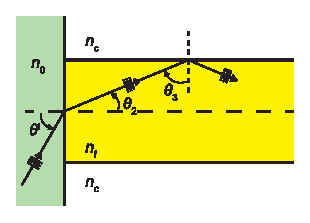
\includegraphics[width=2in]{modules/m0192_fAA.eps} 
% https://commons.wikimedia.org/wiki/File:Injecting_Light_into_Optical_Fiber.svg
}}{A plane wave travels through a medium (n subscript zero) at an angle theta superscript i before entering a fiber optic cable at its center. The wave travels through the fiber (n subscript f) at an angle theta subscript 2 and hits the edge at an angle of theta subscript 3 measured from the vertical. The wave reflects back into the fiber. Area outside the fiber is n subscript c.}
\end{center}
\centerline{\scriptsize 
\copyright~\hyperref[m0192_fAA_Credit]{S.\ Lally} 
\href{https://creativecommons.org/licenses/by-sa/4.0/}{CC BY-SA 4.0} 
} % \centerline 
\caption{
\label{m0192_fAA}
Injecting light into a fiber optic cable.
}
\end{figure} 
%
In this figure, we see light incident from a medium having index of refraction $n_0$, with angle of incidence $\theta^i$.
The light is transmitted with angle of transmission $\theta_2$ into the fiber, and is subsequently incident on the surface of the cladding with angle of incidence $\theta_3$.
For light to propagate without loss within the cable, it is required that 
%
\begin{equation}
\sin\theta_3 \ge \frac{n_c}{n_f}
\label{m0192_eCAnm}
\end{equation}
%
since this criterion must be met in order for total internal reflection to occur.

Now consider the constraint that Equation~\ref{m0192_eCAnm} imposes on $\theta^i$.
First, we note that $\theta_3$ is related to $\theta_2$ as follows:
%
\begin{equation}
\theta_3 = \frac{\pi}{2} - \theta_2
\end{equation} 
%
therefore
%
\begin{flalign}
\sin\theta_3 &= \sin\left(\frac{\pi}{2} - \theta_2\right) \\
             &= \cos\theta_2 
\end{flalign} 
%
so
%
\begin{equation}
\cos\theta_2 \ge \frac{n_c}{n_f}
\end{equation}
%
Squaring both sides, we find: 
%
\begin{equation}
\cos^2\theta_2 \ge \frac{n_c^2}{n_f^2}
\end{equation}
%
Now invoking a trigonometric identity:
%
\begin{equation}
1-\sin^2\theta_2 \ge \frac{n_c^2}{n_f^2}
\end{equation}
%
so:
%
\begin{equation}
\sin^2\theta_2 \le 1-\frac{n_c^2}{n_f^2}
\label{m0192_e1}
\end{equation}
%
Now we relate the $\theta_2$ to $\theta^i$ using Snell's law:
\index{Snell's law}
%
\begin{equation}
\sin\theta_2 = \frac{n_0}{n_f}\sin\theta^i
\end{equation}
%
so Equation~\ref{m0192_e1} may be written:
%
\begin{equation}
\frac{n_0^2}{n_f^2}\sin^2\theta^i \le 1-\frac{n_c^2}{n_f^2}
\end{equation}
%
Now solving for $\sin\theta^i$, we obtain:
%
\begin{equation}
\sin\theta^i \le \frac{1}{n_0}\sqrt{ n_f^2 - n_c^2 }
\end{equation}
%
This result indicates the range of angles of incidence which result in total internal reflection within the fiber.
The maximum value of $\theta^i$ which satisfies this condition is known as the \emph{acceptance angle} 
\index{acceptance angle}
$\theta_a$, so:
%
\begin{equation}
\theta_a \triangleq \arcsin\left(\frac{1}{n_0}\sqrt{ n_f^2 - n_c^2 }\right)
\end{equation}
%
This leads to the following insight:  
%
%%%%%%%%%%%%%%%%%%%%%%%%%%%%%%%%%%%%%%%%%%%%%%%
%ORB HIGHLIGHT
\begin{mdframed}[backgroundcolor=yellow!20,nobreak=true] 
In order to effectively launch light in the fiber, it is necessary for the light to arrive from within a cone having half-angle $\theta_a$ with respect to the axis of the fiber.
\end{mdframed}
%%%%%%%%%%%%%%%%%%%%%%%%%%%%%%%%%%%%%%%%%%%%%%%
%
The associated \emph{cone of acceptance}
\index{cone of acceptance}
is illustrated in Figure~\ref{m0192_fAcceptanceAngle}.
%
\begin{figure}[b!] % <--- "[b]" for first figure in section *only*; delete for 2nd and subsequent figures
\begin{center}
\pdftooltip{{  % note double braces
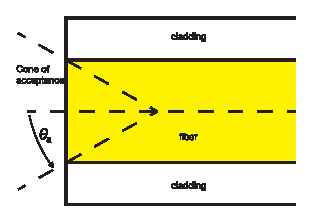
\includegraphics[width=\columnwidth]{modules/m0192_fAcceptanceAngle.eps} 
% https://commons.wikimedia.org/wiki/File:Cone_of_Acceptance.svg
}}{A cross-section of optical fiber with exterior cladding. The cone of acceptance appears as a triangle centered around the axis of the cable. The maximum angle from center is theta subscript a.}
\end{center}
\centerline{\scriptsize 
\copyright~\hyperref[m0192_fAcceptanceAngle_Credit]{S.\ Lally} 
\href{https://creativecommons.org/licenses/by-sa/4.0/}{CC BY-SA 4.0} 
} % \centerline 
\caption{
\label{m0192_fAcceptanceAngle}
Cone of acceptance.
}
\end{figure} 

It is also common to define the quantity \emph{numerical aperture} 
\index{numerical aperture}
NA as follows:
%
\begin{equation}
\mbox{NA} \triangleq \frac{1}{n_0}\sqrt{ n_f^2 - n_c^2 }
\label{m0192_eNA}
\end{equation}
%
Note that $n_0$ is typically very close to $1$ (corresponding to incidence from air), so it is common to see NA defined as simply $\sqrt{ n_f^2 - n_c^2 }$.
This parameter is commonly used in lieu of the acceptance angle in datasheets for fiber optic cable.

%%%%%%%%%%%%%%%%%%%%%%%%%%%%%%%%%%%%%%%%%%%%%%%
%ORB EXAMPLE
~\\ \begin{example} 
\begin{mdframed}[backgroundcolor=brown!20,linecolor=brown!20]\raggedright
Acceptance angle.
\\~\\
Typical values of $n_f$ and $n_c$ for an optical fiber are 1.52 and 1.49, respectively.  What are the numerical aperture and the acceptance angle?

{\bf Solution}. 
Using Equation~\ref{m0192_eNA} and presuming $n_0=1$, we find NA $\cong \underline{0.30}$.
Since $\sin\theta_a =$ NA, we find $\theta_a=\underline{17.5^{\circ}}$.
Light must arrive from within $17.5^{\circ}$ from the axis of the fiber in order to ensure total internal reflection within the fiber.
\end{mdframed}
% note figures will need to go between "\end{mdframed}" and "\end{example}"
\end{example}
%%%%%%%%%%%%%%%%%%%%%%%%%%%%%%%%%%%%%%%%%%%%%%%


%%%%%%%%%%%%%%%%%%%%%

{\bf Additional Reading:}
\begin{itemize}
\item ``\href{https://en.wikipedia.org/wiki/Optical_fiber}{Optical fiber}'' on Wikipedia.
\item ``\href{https://en.wikipedia.org/wiki/Numerical_aperture}{Numerical aperture}'' on Wikipedia.
\end{itemize}

\index{optical fiber|)}


